\def\Title{\hfill \huge{コミュニケーション/メディア概念と関連付けた情報概念の形式化} \hfill}
\def\Author{大西 洋 (京都市立西京高校)}
\include{myposter}
\include{embed}
\definecolor{em-bg}{rgb}{0.8, 1.0, 0.8}

\bibliography{poster-zen2018}
\nocite{*}
\Header

\section{Background}
\begin{columns}[onlytextwidth,t]
\begin{column}{.5\hsize}
\begin{block}{\insertsection}
\alert{情報}概念を体系的に扱う\em{基礎情報学}\cite{nishigaki1}\cite{nishigaki2}\cite{nishigaki3}に基づく授業を実践\cite{ohnishi}
\begin{itemize}
\item 情報(information ← \alert{in} + \alert{form})をパターンとして定義 \\ 西垣「それによって生物がパターンをつくりだすパターン」\cite{nishigaki1}
\item 情報の解釈は生命に特有(\em{生命情報}・意味作用)
\item 意味は客観的に定まるものではない \\ (情報の\em{主観性}:「情報は伝わらない」)
\item 記号と意味内容が一体化してコミュニケーションが可能に(\em{社会情報})
\item 意味内容の潜在化により機械が情報を処理(複製)可能に(\em{機械情報})
\item 「\em{情報量}」(bit)はあくまで記号の数で、意味の「大きさ」(価値)は測れない
\item コミュニケーションやメディアの概念と接続
\end{itemize}
\end{block}
\end{column}
\begin{column}{.47\hsize}
\begin{figure}[hbtp]{\centering
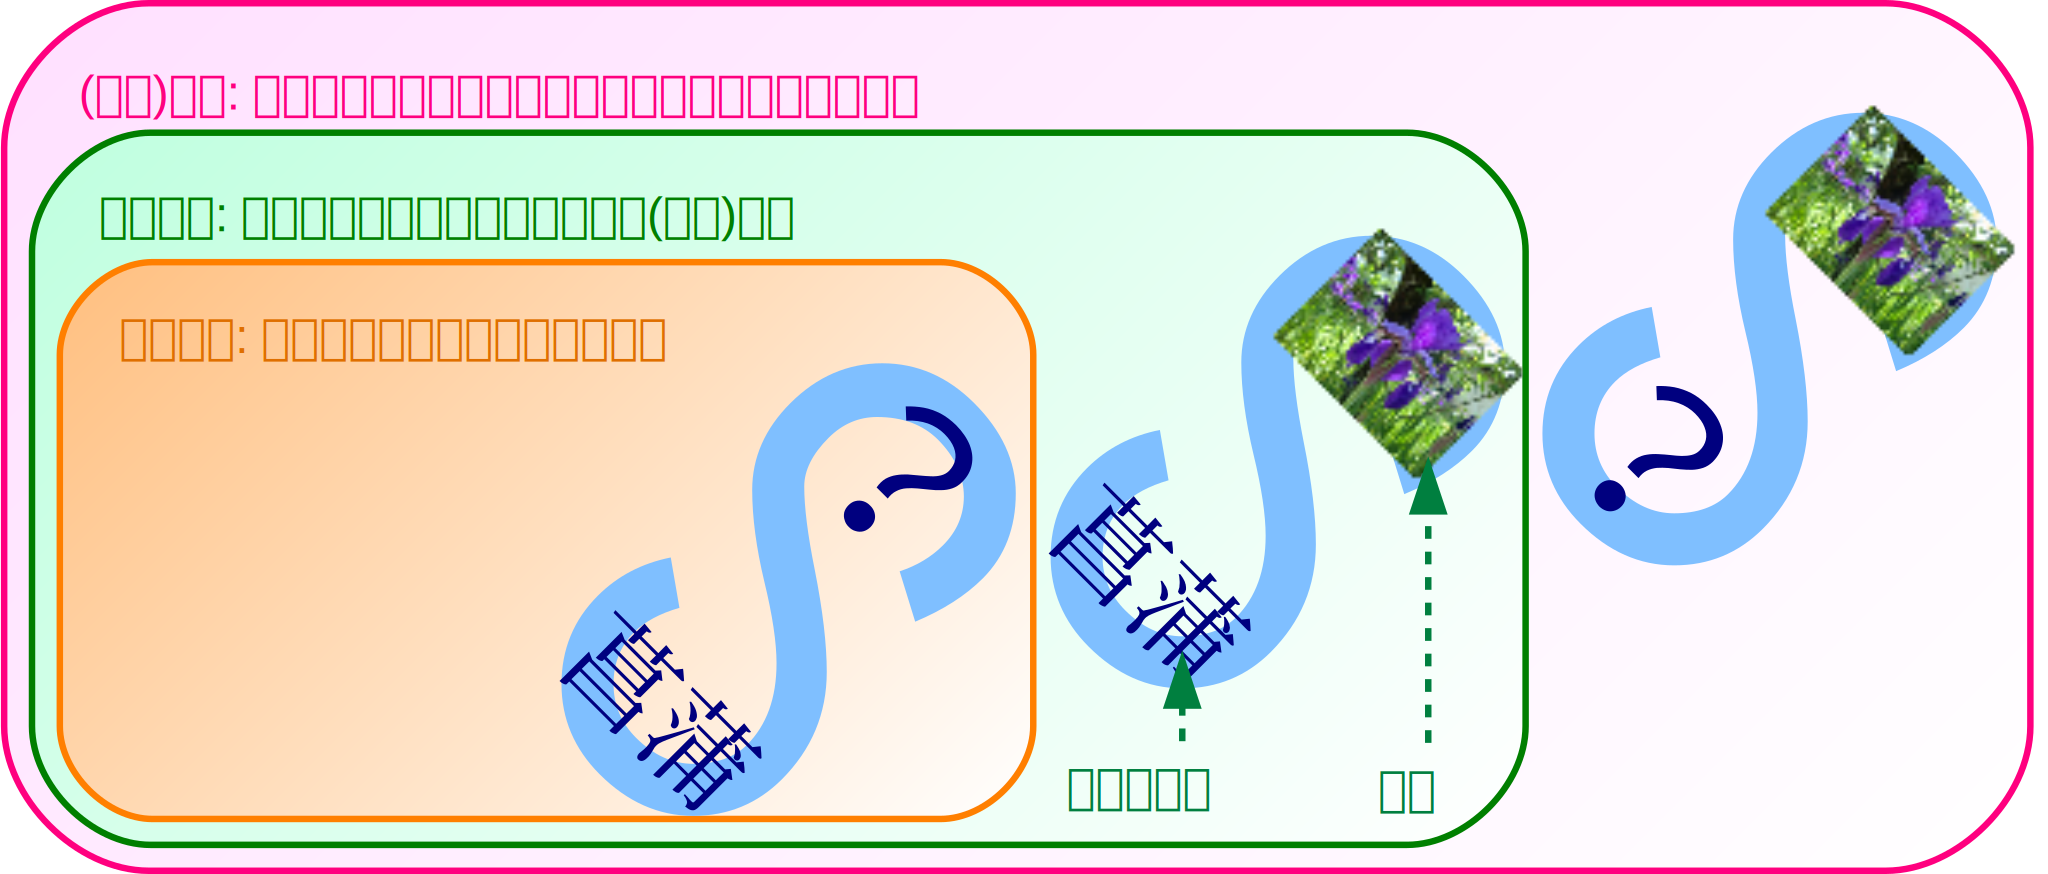
\includegraphics[scale=2.5]{inclusion2-org.pdf}
\caption{基礎情報学における3種の情報概念}
}\end{figure}
\end{column}
\end{columns}

\begin{columns}[onlytextwidth,t]
\begin{column}{.5\hsize}
\begin{block}{Problem}
基礎情報学の理論上の課題
\begin{itemize}
\item 3つの情報の\em{包含関係}は適切か? \\ 「パターンをつくりだす」生命情報の中に「意味内容が潜在化した(=パターンを生じさせない)」機械情報がある?
\item 「情報」の\em{日常的用法}との乖離 \\ e.g.「情報通信」「情報交換」「情報発信」
\item 各概念の定義に\em{曖昧性}がある \\ (コミュニケーション/メディアの理論との接続が難しい)
\item Saussureの\em{記号論}\cite{saussure}との接続が弱い(言語学の理論と分断)
\item 「\em{パターン}」の定義が不明瞭
\end{itemize}
\end{block}
\end{column}
\begin{column}{.47\hsize}
\begin{figure}[hbtp]{\centering
\includegraphics[scale=1.5]{model-comm.pdf}
\caption{情報/コミュニケーション/メディアの接続\cite{ohnishi}}
}\end{figure}
\end{column}
\end{columns}

\section{Proposal}
\begin{columns}[onlytextwidth,t]
\begin{column}{.5\hsize}
\begin{alertblock}{Research Purpose}
数学的表現を用いて\alert{「情報」概念を再定義}し、\em{厳密化}・\em{形式化}する
\begin{itemize}
	\item 基礎情報学を基にしつつ、\em{Saussure}の記号論との接続を強化
	\item \em{コミュニケーション}/\em{メディア}の理論との接続を志向
\end{itemize}
\end{alertblock}
\end{column}
\begin{column}{.47\hsize}
\begin{block}{encode/decode}
Hallのモデル\cite{hall}\cite{hall2}を基に形式化
\begin{itemize}
	\item \alert{encode}(符号化): 意味$\beta$に対応する\em{記号$\alpha$を生成}する操作($\alpha = e(\beta)$)
	\item \alert{decode}(復号): 記号$\alpha$に対応する\em{意味$\beta$を生成}する操作($\beta = d(\alpha)$)
	\item[※] 情報の\em{主観性}により、$\alpha = e(d(\alpha)), \beta = d(e(\beta))$とは限らない($d \neq e^{-1}$)
\end{itemize}
\end{block}
\end{column}
\end{columns}

\begin{columns}[onlytextwidth,t]
\begin{column}{.24\hsize}
\begin{block}{「情報」概念の形式的定義}
\alert{情報}を$\alpha$と$\beta$の組$I := (\alpha, \beta)$と定義
\begin{itemize}
	\item $\alpha$: \alert{記号}(その情報を表す表現)
	\item $\beta $: \alert{意味}(その情報が表す概念)
	\item $\alpha, \beta$のいずれかを\em{空列}($\varepsilon$)とすることも可能
	\item[※] Saussureの語法では、$I$は記号、 \\
		$\alpha$は記号表現(signifiant, 能記)、 \\
		$\beta$は記号内容(signifié, 所記)\cite{saussure}
\end{itemize}
\end{block}
\end{column}
\begin{column}{.24\hsize}
\begin{block}{「情報」概念の分類}
\begin{itemize}
	\item $\alpha = \varepsilon$のとき$I$を\alert{生命情報}と呼ぶ \\ (表現を持たない情報は、生命の内部でのみ存在可能)
	\item $\beta  = \varepsilon$のとき$I$を\alert{機械情報}と呼ぶ \\ (意味を持たない情報は、機械でも処理可能)
	\item それ以外のとき$I$を\alert{社会情報}と呼ぶ ($\alpha$と$\beta$の対応により、生命の社会が成立可能)
\end{itemize}
\end{block}
\end{column}
\begin{column}{.47\hsize}
\begin{block}{コミュニケーション・モデルの形式化}
送り手$i$から受け手$j$へのコミュニケーションを想定する\cite{luhmann}\cite{borch}\cite{ohnishi}
\begin{enumerate}
	\item \alert{情報の選択} \\
		送り手$i$が伝えたい\em{生命情報}$(\varepsilon, \beta)$が選択される
	\item \alert{表現の選択} \\
		\em{生命情報}$(\varepsilon, \beta)$が送り手$i$によりencodeされて\em{社会情報}$(e_i(\beta), \beta)$になる
	\item \alert{理解の選択} \\
		\em{機械情報}$(\alpha, \varepsilon)$が受け手$j$によりdecodeされて\em{社会情報}$(\alpha, d_j(\alpha))$になる
	\item \alert{理解の受容の選択} \\
		\em{社会情報}$(\alpha, d(\alpha))$の意味$d(\alpha)$を受け手$j$が受け入れるかが選択される \\
		(受け手$j$の内部で生命情報$(\varepsilon, \beta')$が生起する)
\end{enumerate}
\end{block}
\end{column}
\end{columns}

\begin{columns}[onlytextwidth,t]
\begin{column}{.5\hsize}
\begin{figure}[hbtp]{\centering
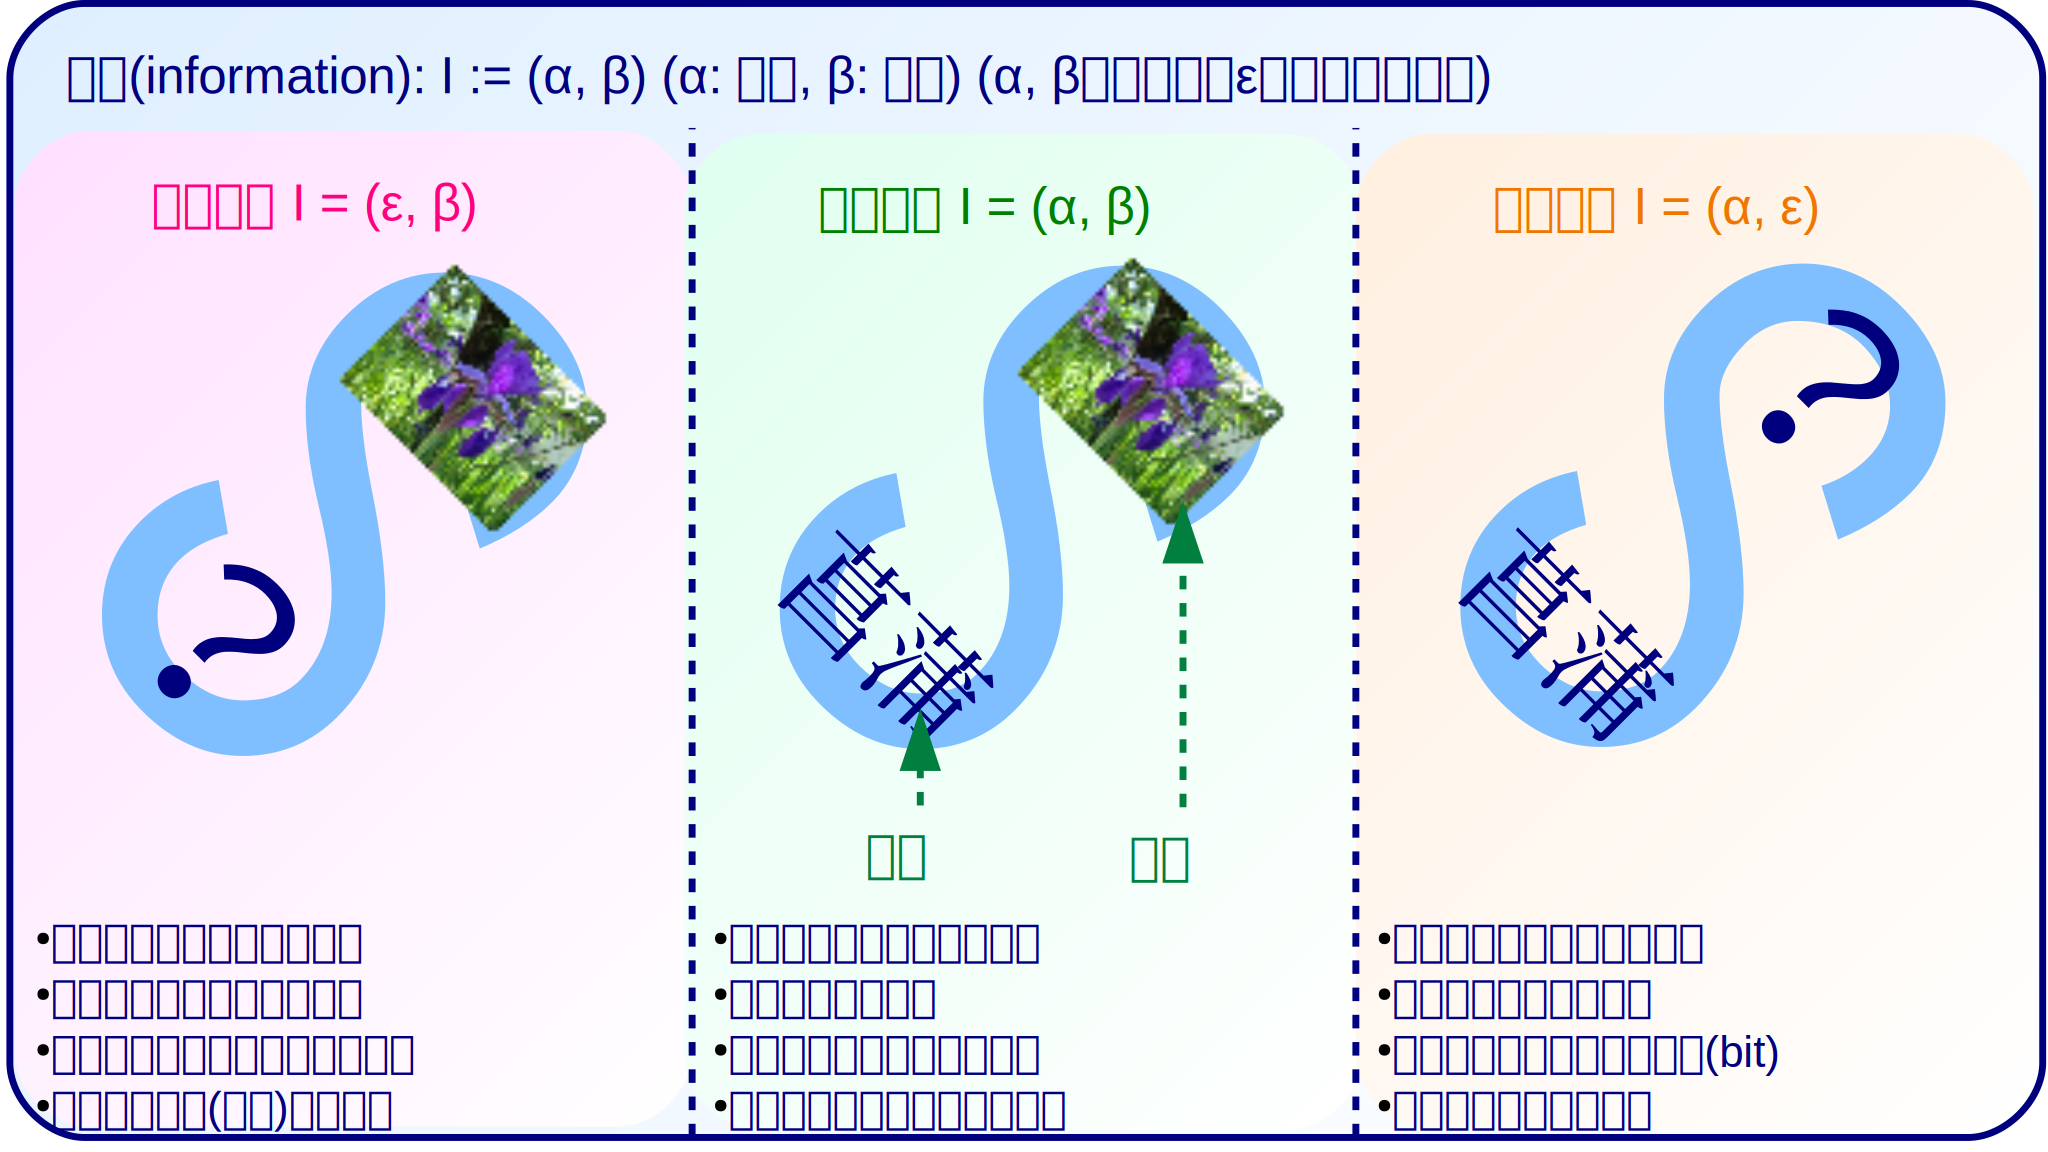
\includegraphics[scale=2.5]{information.pdf}
\caption{提案する情報概念}
}\end{figure}
\end{column}
\begin{column}{.47\hsize}
\begin{block}{メディアの形式化}
Luhmannによるメディア概念\cite{borch}\cite{nishigaki1}を形式化 \\
(「ありそうもない(\em{unlikely})」ことを「ありうる(\em{likely})」ことにする機構)
\begin{itemize}
	\item \alert{伝播メディア}: \em{機械情報}を\em{物理的}に媒介 \\
		選択された表現が受け手に到達することを媒介 \\
		($\alpha = e_i(\beta)$の成立可能性を高める)
	\item \alert{成果メディア}: \em{社会情報}を\em{論理的}に媒介 \\
		選択された理解が受け手に受け入れられることを媒介 \\
		($\beta' = \beta$の成立可能性を高める)
	\item[※] 言語(集団語, jargon): (Luhmannはメディアに分類) \\
		(社会情報の部分集合$L$の要素$(\alpha, \beta)$について、$\alpha = e(\beta), \beta = d(\alpha)$) \\
		($\beta = d_j(e_i(\beta))$の成立可能性を高める)
\end{itemize}
\end{block}
\end{column}
\end{columns}

\section{Conclusion}
\begin{columns}[onlytextwidth,t]
\begin{column}{.3\hsize}
\begin{block}{\insertsection}
	\begin{itemize}
		\item 情報概念を\em{形式化}することで曖昧性を低減
		\item 情報/コミュニケーション/メディアを統一的に議論するための\em{理論的基礎}を構築
	\end{itemize}
\end{block}

\begin{block}{Future Tasks}
	\begin{itemize}
		\item 言語とメディアの関係性の検討
		\item 生徒向け教材・資料の整備
		\item 本発表の枠組みに基づく授業の実践と評価
	\end{itemize}
\end{block}
\end{column}
\begin{column}{.67\hsize}
\begin{block}{References}
\renewcommand*{\bibfont}{\scriptsize}
\printbibliography
\end{block}
\end{column}
\end{columns}

\end{frame}
\end{document}
